\documentclass[border=4pt,12pt]{standalone}
% House style for redrawn exam diagrams (diagram-v4: 0.4pt lines, filled -latex arrows, fine dashes; stipple and hatching drawn as real dots/lines (no PDF/SVG patterns, so they render in every browser and at any scale); transparent background). Every figure \input's this.
\usepackage{amsmath,amssymb}
\usepackage{txfonts}
\usepackage{pdfrender,xcolor}
% \halo{text}: label on shading. The shading stops just around each letter's outline (a thin knock-out that follows the
% glyphs, like the papers' typesetting), never a box. Owner: "I don't want a box around the text".
\newcommand{\halo}[1]{\leavevmode\rlap{\pdfrender{TextRenderingMode=2,LineWidth=2.2pt,LineJoinStyle=1,StrokeColor=white,FillColor=white}#1}#1}
\usepackage{tikz,pgfplots}
\pgfplotsset{compat=1.18}
\usetikzlibrary{arrows.meta,calc,angles,quotes,patterns,patterns.meta,intersections,positioning,decorations.markings,shapes.geometric}
% Stipple and hatching are drawn as actual dots / lines clipped to the region (path picture), NOT as pattern fills:
% SVG <pattern> fills vanish or blur when browsers scale the image, so the owner could not see the shading.
% Each dot is a 0.72pt square (keeps SVGs small; reads as a dot at print size). Dots sit on one global staggered grid, so neighbouring regions line up.
\makeatletter
\newdimen\ex@x \newdimen\ex@y \newdimen\ex@xa \newdimen\ex@ya \newdimen\ex@xb \newdimen\ex@yb \newcount\ex@row
\def\exam@stipplecolor{black!75}\def\exam@dotr{0.42pt}\def\exam@dotgap{2.5}
\def\ex@rowdots{\ifdim\ex@x<\ex@xb \pgfpathrectangle{\pgfqpoint{\dimexpr\ex@x-0.36pt\relax}{\dimexpr\ex@y-0.36pt\relax}}{\pgfqpoint{0.72pt}{0.72pt}}\advance\ex@x by \exam@dotgap pt\relax\expandafter\ex@rowdots\fi}
\def\exam@stipple{%
  \pgftransformreset% dots are sized in real points even inside scaled pictures
  \pgfpointanchor{path picture bounding box}{south west}\ex@xa=\pgf@x \ex@ya=\pgf@y
  \pgfpointanchor{path picture bounding box}{north east}\ex@xb=\pgf@x \ex@yb=\pgf@y
  \pgfsetfillcolor{\exam@stipplecolor}\pgfmathsetmacro\ex@h{\exam@dotgap/2}%
  \pgfmathtruncatemacro\ex@r{floor(\ex@ya/\ex@h)-1}\ex@row=\ex@r\relax
  \ex@y=\ex@r\dimexpr\ex@h pt\relax
  \loop\ifdim\ex@y<\ex@yb
    \pgfmathtruncatemacro\ex@c{floor(\ex@xa/\exam@dotgap)-1}\ex@x=\ex@c\dimexpr\exam@dotgap pt\relax
    \ifodd\ex@row \advance\ex@x by \ex@h pt\fi
    \ex@rowdots
    \advance\ex@y by \ex@h pt \advance\ex@row by 1
    \ifnum\numexpr\ex@row-(\ex@row/4)*4\relax=0 \pgfusepath{fill}\fi% flush every 4 rows: bounded TeX memory, few clip copies in the SVG
  \repeat\pgfusepath{fill}}
\newdimen\ex@d
\def\exam@hatch#1{% #1 = 1 for /, -1 for \ ; lines 45 degrees, 3pt apart
  \pgftransformreset
  \pgfpointanchor{path picture bounding box}{south west}\ex@xa=\pgf@x \ex@ya=\pgf@y
  \pgfpointanchor{path picture bounding box}{north east}\ex@xb=\pgf@x \ex@yb=\pgf@y
  \ex@d=\dimexpr\ex@yb-\ex@ya\relax \ex@x=\dimexpr\ex@xa-\ex@d\relax
  \loop\ifdim\ex@x<\ex@xb
    \ifnum#1>0 \pgfpathmoveto{\pgfqpoint{\ex@x}{\ex@ya}}\pgfpathlineto{\pgfqpoint{\dimexpr\ex@x+\ex@d\relax}{\ex@yb}}%
    \else \pgfpathmoveto{\pgfqpoint{\ex@x}{\ex@yb}}\pgfpathlineto{\pgfqpoint{\dimexpr\ex@x+\ex@d\relax}{\ex@ya}}\fi
    \advance\ex@x by 4.24pt
  \repeat
  \pgfsetlinewidth{0.4pt}\pgfsetstrokecolor{black}\pgfusepath{stroke}}
\def\examstipple{\exam@stipple}\def\examhatch{\exam@hatch}\def\examsetstipplecolor#1{\def\exam@stipplecolor{#1}}\def\examsetdotgap#1{\def\exam@dotgap{#1}}
\makeatother
% (legacy pattern kept for old files)
% staggered stipple like the NESA papers' dotted shading
\pgfdeclarepatternformonly{exam stipple}{\pgfpointorigin}{\pgfqpoint{2.2pt}{2.2pt}}{\pgfqpoint{2.2pt}{2.2pt}}{%
  \pgfpathcircle{\pgfqpoint{0.55pt}{0.55pt}}{0.42pt}\pgfpathcircle{\pgfqpoint{1.65pt}{1.65pt}}{0.42pt}\pgfusepath{fill}}
\tikzset{
  every picture/.style={line width=0.6pt, >={Latex[length=2mm,width=1.3mm]}},
  curve/.style={line width=0.6pt},
  open arrow/.style={-{Latex[length=2mm,width=1.3mm]}},  % owner: filled -latex heads everywhere, no open chevrons
  aux/.style={dash pattern=on 2pt off 1.5pt, line width=0.6pt},
  shade/.code={\def\exA{#1}\def\exB{none}\ifx\exA\exB\else\pgfkeysalso{fill=black!18}\fi},
  shade/.default=on,
  shade dots/.style={fill=none, path picture={\examstipple}},
  stipple color/.code={\examsetstipplecolor{#1}},
  stipple gap/.code={\examsetdotgap{#1}},
  shade dense dots/.style={fill=none, stipple gap=1.6, path picture={\examstipple}},
  shade hatch/.style={fill=none, path picture={\examhatch{1}}},
  shade hatch reverse/.style={fill=none, path picture={\examhatch{-1}}},
  shade solid/.style={fill=black},
  pt/.style={circle, fill, inner sep=1.1pt},
  open pt/.style={circle, draw, fill=white, inner sep=1.1pt},
}
\pgfplotsset{
  exam axes/.style={axis lines=middle, axis line style={->}, xlabel={$x$}, ylabel={$y$},
    xlabel style={anchor=west}, ylabel style={anchor=south}, tick label style={font=\small},
    every axis plot/.append style={line width=0.6pt, black}, samples=200, clip=false,
    enlargelimits=false, axis on top},
}

\usetikzlibrary{decorations.pathreplacing}
\begin{document}
% 2025 Fort Street AT4 Q32 solution: trapezium ABCD (AB=4, CD=2, base angles 60 deg, h=sqrt3), feet E, H, F of the
% perpendiculars from D, P, C. Clean redraw consistent with the worked solution (rules 16-18); theta arc and label
% clear of AP, AB, the AE tick and the DE dashed line (owner: "the theta is overlapping"; rules 11, 14).
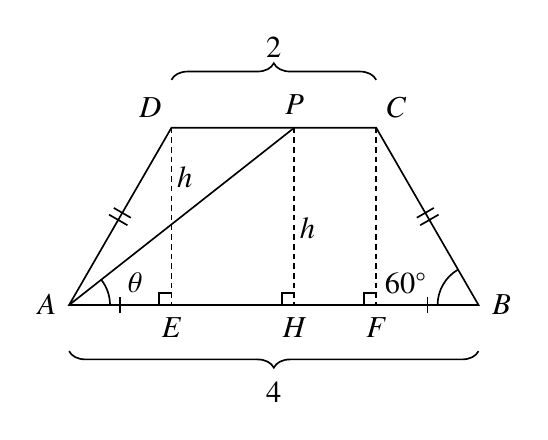
\begin{tikzpicture}[x=1.3cm,y=1.3cm,every node/.style={font=\fontsize{11}{13}\selectfont}]
  \coordinate (A) at (0,0); \coordinate (B) at (4,0); \coordinate (C) at (3,1.732); \coordinate (D) at (1,1.732);
  \coordinate (P) at (2.2,1.732); \coordinate (E) at (1,0); \coordinate (H) at (2.2,0); \coordinate (F) at (3,0);
  \draw (A) -- (B) -- (C) -- (D) -- cycle;
  \draw (A) -- (P);
  \draw[aux] (D) -- (E); \draw[aux] (P) -- (H); \draw[aux] (C) -- (F);
  % AD = BC (double ticks), AE = FB (single ticks)
  \foreach \s/\t in {A/D,B/C}{
    \path ($(\s)!0.5!(\t)$) coordinate (M) ($(\s)!0.5!(\t)!0.07!90:(\t)$) coordinate (N);
    \draw ($(M)!0.04!(\t)!0.1!90:(\t)$) -- ($(M)!0.04!(\t)!0.1!-90:(\t)$);
    \draw ($(M)!-0.04!(\t)!0.1!90:(\t)$) -- ($(M)!-0.04!(\t)!0.1!-90:(\t)$);}
  \draw (0.5,-0.08) -- (0.5,0.08); \draw (3.5,-0.08) -- (3.5,0.08);
  % right angles at E, H, F
  \foreach \q in {E,H,F}{\draw ($(\q)+(-0.12,0)$) -- ++(0,0.12) -- ++(0.12,0);}
  % angles
  \draw (0.4,0) arc[start angle=0,end angle=38.2,radius=0.4];
  \node at (19.1:0.68) {$\theta$};
  \draw (3.6,0) arc[start angle=180,end angle=120,radius=0.4];
  \node at ($(B)+(163:0.74)$) {$60^\circ$};
  % heights
  \node at (1.13,1.25) {$h$};
  \node at (2.33,0.75) {$h$};
  % lengths
  \draw[decorate,decoration={brace,amplitude=6pt}] (1,2.2) -- (3,2.2);
  \node at (2,2.52) {$2$};
  \draw[decorate,decoration={brace,amplitude=6pt,mirror}] (0,-0.45) -- (4,-0.45);
  \node at (2,-0.85) {$4$};
  % vertex labels
  \node[above left=0pt] at (D) {$D$}; \node[above=1pt] at (P) {$P$}; \node[above right=0pt] at (C) {$C$};
  \node[left=1pt] at (A) {$A$}; \node[right=1pt] at (B) {$B$};
  \node[below=1pt] at (E) {$E$}; \node[below=1pt] at (H) {$H$}; \node[below=1pt] at (F) {$F$};
\end{tikzpicture}
\end{document}
